\documentclass{article}
\usepackage[paperwidth=6.5in,paperheight=7.6in,margin=0in]{geometry}
\usepackage{tikz,fix-cm,amsmath,amssymb}
\pagestyle{empty}
\definecolor{blue}{HTML}{276185}
\definecolor{red}{HTML}{AD3E35}
\definecolor{ink}{HTML}{262626}
\definecolor{gray}{HTML}{666666}
\definecolor{green}{HTML}{35734A}
\begin{document}\noindent\sffamily
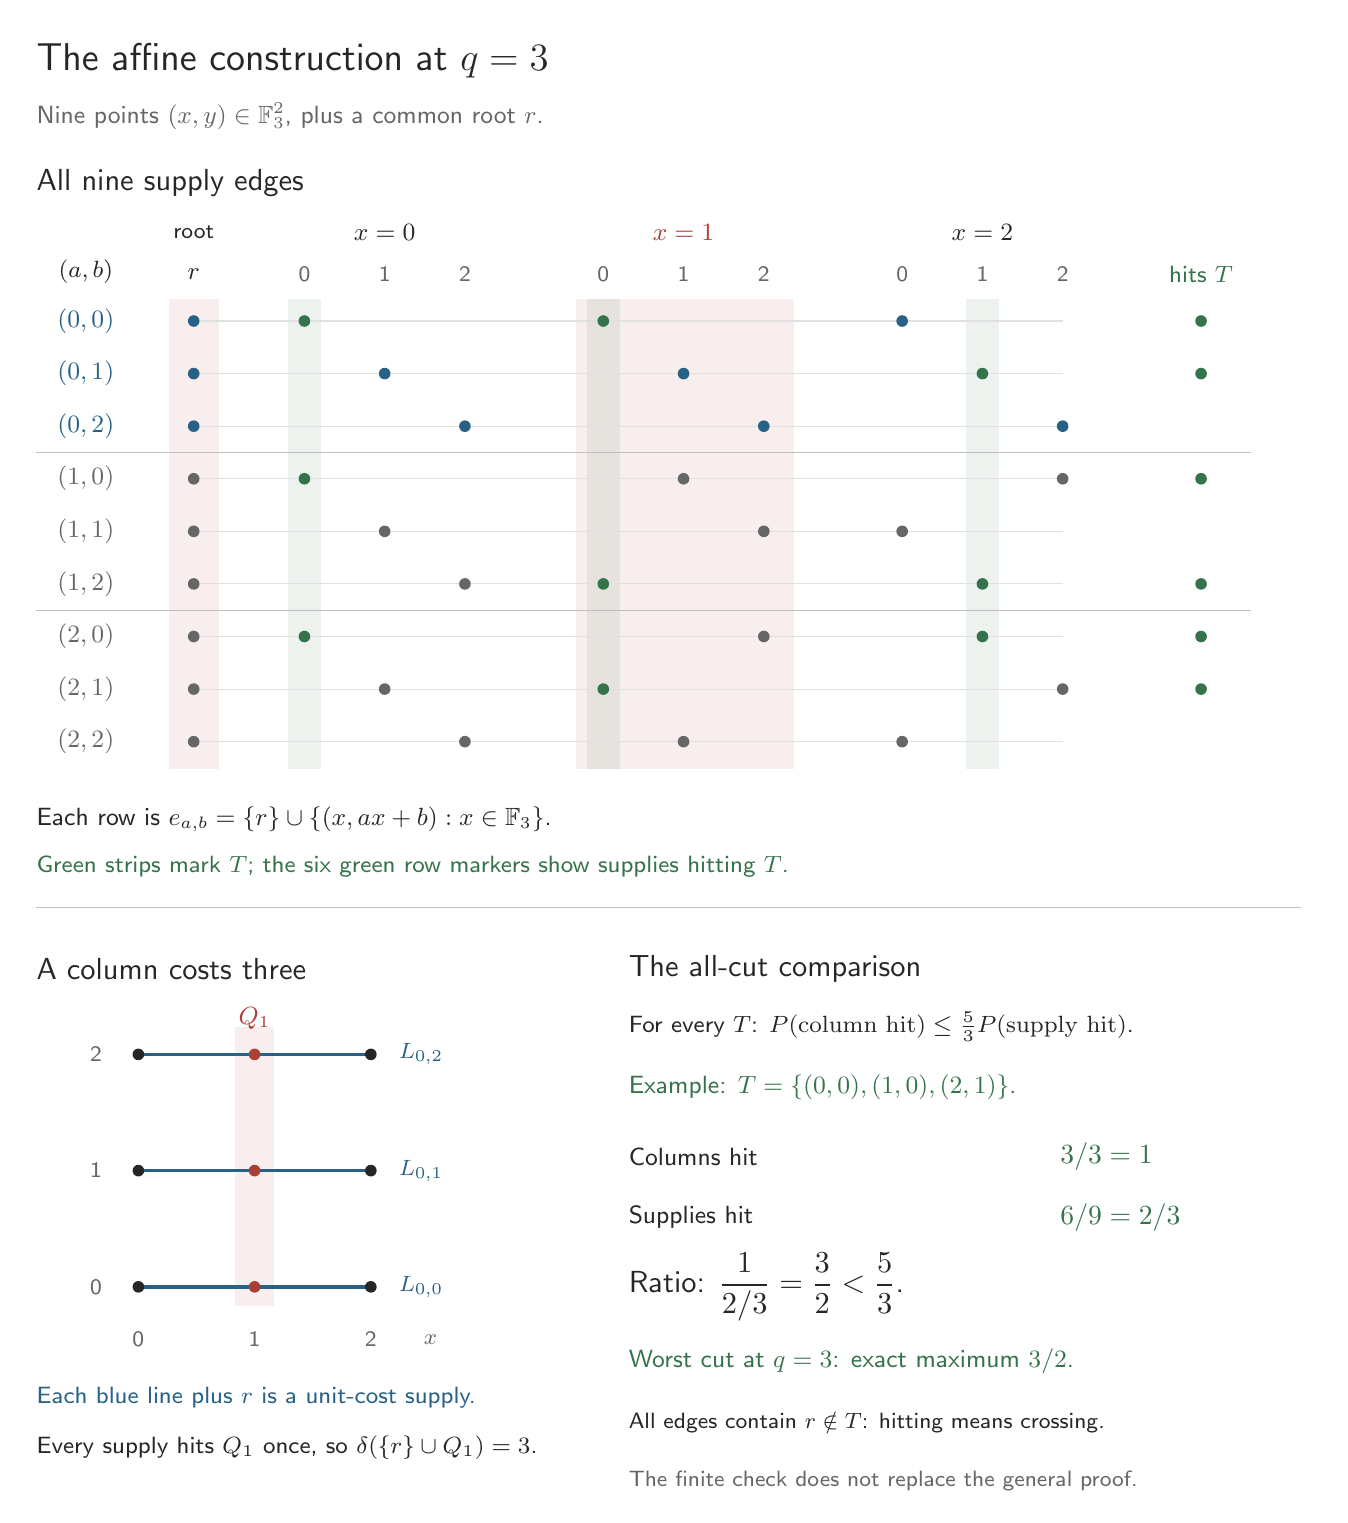
\begin{tikzpicture}[x=1pt,y=-1pt,every node/.style={inner sep=0pt,text=ink}]
\path[use as bounding box] (0,0) rectangle (467,530);

\node[anchor=west,text=ink,font=\sffamily\fontsize{14}{18.2}\selectfont] at (3,12) {The affine construction at $q=3$};
\node[anchor=west,text=gray,font=\sffamily\fontsize{9}{11.700000000000001}\selectfont] at (3,32) {Nine points $(x,y)\in\mathbb F_3^2$, plus a common root $r$.};
\node[anchor=west,text=ink,font=\sffamily\fontsize{11}{14.3}\selectfont] at (3,56) {All nine supply edges};
\fill[red,opacity=.09] (51,98) rectangle (69,268);
\fill[red,opacity=.09] (198,98) rectangle (277,268);
\fill[green,opacity=.09] (94,98) rectangle (106,268);
\fill[green,opacity=.09] (202,98) rectangle (214,268);
\fill[green,opacity=.09] (339,98) rectangle (351,268);
\node[anchor=center,text=ink,font=\sffamily\fontsize{8.5}{11.05}\selectfont] at (21,88) {$(a,b)$};
\node[anchor=center,text=ink,font=\sffamily\fontsize{8}{10.4}\selectfont] at (60,74) {root};
\node[anchor=center,text=ink,font=\sffamily\fontsize{9}{11.700000000000001}\selectfont] at (60,89) {$r$};
\node[anchor=center,text=ink,font=\sffamily\fontsize{9}{11.700000000000001}\selectfont] at (129,74) {$x=0$};
\node[anchor=center,text=gray,font=\sffamily\fontsize{8}{10.4}\selectfont] at (100,89) {0};
\node[anchor=center,text=gray,font=\sffamily\fontsize{8}{10.4}\selectfont] at (129,89) {1};
\node[anchor=center,text=gray,font=\sffamily\fontsize{8}{10.4}\selectfont] at (158,89) {2};
\node[anchor=center,text=red,font=\sffamily\fontsize{9}{11.700000000000001}\selectfont] at (237,74) {$x=1$};
\node[anchor=center,text=gray,font=\sffamily\fontsize{8}{10.4}\selectfont] at (208,89) {0};
\node[anchor=center,text=gray,font=\sffamily\fontsize{8}{10.4}\selectfont] at (237,89) {1};
\node[anchor=center,text=gray,font=\sffamily\fontsize{8}{10.4}\selectfont] at (266,89) {2};
\node[anchor=center,text=ink,font=\sffamily\fontsize{9}{11.700000000000001}\selectfont] at (345,74) {$x=2$};
\node[anchor=center,text=gray,font=\sffamily\fontsize{8}{10.4}\selectfont] at (316,89) {0};
\node[anchor=center,text=gray,font=\sffamily\fontsize{8}{10.4}\selectfont] at (345,89) {1};
\node[anchor=center,text=gray,font=\sffamily\fontsize{8}{10.4}\selectfont] at (374,89) {2};
\node[anchor=center,text=green,font=\sffamily\fontsize{8.5}{11.05}\selectfont] at (424,89) {hits $T$};
\draw[black!12,line width=0.4pt] (60,106)--(374,106);
\node[anchor=center,text=blue,font=\sffamily\fontsize{9}{11.700000000000001}\selectfont] at (21,106) {$(0,0)$};
\fill[blue] (60,106) circle (2.1pt);
\fill[green] (100,106) circle (2.1pt);
\fill[green] (208,106) circle (2.1pt);
\fill[blue] (316,106) circle (2.1pt);
\fill[green] (424,106) circle (2.1pt);
\draw[black!12,line width=0.4pt] (60,125)--(374,125);
\node[anchor=center,text=blue,font=\sffamily\fontsize{9}{11.700000000000001}\selectfont] at (21,125) {$(0,1)$};
\fill[blue] (60,125) circle (2.1pt);
\fill[blue] (129,125) circle (2.1pt);
\fill[blue] (237,125) circle (2.1pt);
\fill[green] (345,125) circle (2.1pt);
\fill[green] (424,125) circle (2.1pt);
\draw[black!12,line width=0.4pt] (60,144)--(374,144);
\node[anchor=center,text=blue,font=\sffamily\fontsize{9}{11.700000000000001}\selectfont] at (21,144) {$(0,2)$};
\fill[blue] (60,144) circle (2.1pt);
\fill[blue] (158,144) circle (2.1pt);
\fill[blue] (266,144) circle (2.1pt);
\fill[blue] (374,144) circle (2.1pt);
\draw[black!12,line width=0.4pt] (60,163)--(374,163);
\node[anchor=center,text=gray,font=\sffamily\fontsize{9}{11.700000000000001}\selectfont] at (21,163) {$(1,0)$};
\fill[gray] (60,163) circle (2.1pt);
\fill[green] (100,163) circle (2.1pt);
\fill[gray] (237,163) circle (2.1pt);
\fill[gray] (374,163) circle (2.1pt);
\fill[green] (424,163) circle (2.1pt);
\draw[black!12,line width=0.4pt] (60,182)--(374,182);
\node[anchor=center,text=gray,font=\sffamily\fontsize{9}{11.700000000000001}\selectfont] at (21,182) {$(1,1)$};
\fill[gray] (60,182) circle (2.1pt);
\fill[gray] (129,182) circle (2.1pt);
\fill[gray] (266,182) circle (2.1pt);
\fill[gray] (316,182) circle (2.1pt);
\draw[black!12,line width=0.4pt] (60,201)--(374,201);
\node[anchor=center,text=gray,font=\sffamily\fontsize{9}{11.700000000000001}\selectfont] at (21,201) {$(1,2)$};
\fill[gray] (60,201) circle (2.1pt);
\fill[gray] (158,201) circle (2.1pt);
\fill[green] (208,201) circle (2.1pt);
\fill[green] (345,201) circle (2.1pt);
\fill[green] (424,201) circle (2.1pt);
\draw[black!12,line width=0.4pt] (60,220)--(374,220);
\node[anchor=center,text=gray,font=\sffamily\fontsize{9}{11.700000000000001}\selectfont] at (21,220) {$(2,0)$};
\fill[gray] (60,220) circle (2.1pt);
\fill[green] (100,220) circle (2.1pt);
\fill[gray] (266,220) circle (2.1pt);
\fill[green] (345,220) circle (2.1pt);
\fill[green] (424,220) circle (2.1pt);
\draw[black!12,line width=0.4pt] (60,239)--(374,239);
\node[anchor=center,text=gray,font=\sffamily\fontsize{9}{11.700000000000001}\selectfont] at (21,239) {$(2,1)$};
\fill[gray] (60,239) circle (2.1pt);
\fill[gray] (129,239) circle (2.1pt);
\fill[green] (208,239) circle (2.1pt);
\fill[gray] (374,239) circle (2.1pt);
\fill[green] (424,239) circle (2.1pt);
\draw[black!12,line width=0.4pt] (60,258)--(374,258);
\node[anchor=center,text=gray,font=\sffamily\fontsize{9}{11.700000000000001}\selectfont] at (21,258) {$(2,2)$};
\fill[gray] (60,258) circle (2.1pt);
\fill[gray] (158,258) circle (2.1pt);
\fill[gray] (237,258) circle (2.1pt);
\fill[gray] (316,258) circle (2.1pt);
\draw[black!25,line width=0.4pt] (3,153.5)--(442,153.5);
\draw[black!25,line width=0.4pt] (3,210.5)--(442,210.5);
\node[anchor=west,text=ink,font=\sffamily\fontsize{9}{11.700000000000001}\selectfont] at (3,286) {Each row is $e_{a,b}=\{r\}\cup\{(x,ax+b):x\in\mathbb F_3\}$.};
\node[anchor=west,text=green,font=\sffamily\fontsize{8.5}{11.05}\selectfont] at (3,303) {Green strips mark $T$; the six green row markers show supplies hitting $T$.};
\draw[black!25,line width=0.4pt] (3,318)--(460,318);
\node[anchor=west,text=ink,font=\sffamily\fontsize{11}{14.3}\selectfont] at (3,340) {A column costs three};
\node[anchor=west,text=ink,font=\sffamily\fontsize{11}{14.3}\selectfont] at (217,340) {The all-cut comparison};
\node[anchor=west,text=ink,font=\sffamily\fontsize{8.5}{11.05}\selectfont] at (217,361) {For every $T$: $P(\mathrm{column\ hit})\leq\frac53P(\mathrm{supply\ hit})$.};
\node[anchor=west,text=green,font=\sffamily\fontsize{9}{11.700000000000001}\selectfont] at (217,383) {Example: $T=\{(0,0),(1,0),(2,1)\}$.};
\fill[red,opacity=.09] (75,361) rectangle (89,462);
\draw[blue,line width=1.2pt] (40,455)--(124,455);
\fill[ink] (40,455) circle (2.1pt);
\fill[red] (82,455) circle (2.1pt);
\fill[ink] (124,455) circle (2.1pt);
\node[anchor=east,text=gray,font=\sffamily\fontsize{8}{10.4}\selectfont] at (27,455) {0};
\node[anchor=west,text=blue,font=\sffamily\fontsize{8}{10.4}\selectfont] at (134,455) {$L_{0,0}$};
\draw[blue,line width=1.2pt] (40,413)--(124,413);
\fill[ink] (40,413) circle (2.1pt);
\fill[red] (82,413) circle (2.1pt);
\fill[ink] (124,413) circle (2.1pt);
\node[anchor=east,text=gray,font=\sffamily\fontsize{8}{10.4}\selectfont] at (27,413) {1};
\node[anchor=west,text=blue,font=\sffamily\fontsize{8}{10.4}\selectfont] at (134,413) {$L_{0,1}$};
\draw[blue,line width=1.2pt] (40,371)--(124,371);
\fill[ink] (40,371) circle (2.1pt);
\fill[red] (82,371) circle (2.1pt);
\fill[ink] (124,371) circle (2.1pt);
\node[anchor=east,text=gray,font=\sffamily\fontsize{8}{10.4}\selectfont] at (27,371) {2};
\node[anchor=west,text=blue,font=\sffamily\fontsize{8}{10.4}\selectfont] at (134,371) {$L_{0,2}$};
\node[anchor=center,text=gray,font=\sffamily\fontsize{8}{10.4}\selectfont] at (40,474) {0};
\node[anchor=center,text=gray,font=\sffamily\fontsize{8}{10.4}\selectfont] at (82,474) {1};
\node[anchor=center,text=gray,font=\sffamily\fontsize{8}{10.4}\selectfont] at (124,474) {2};
\node[anchor=center,text=red,font=\sffamily\fontsize{9}{11.700000000000001}\selectfont] at (82,358) {$Q_1$};
\node[anchor=west,text=gray,font=\sffamily\fontsize{8}{10.4}\selectfont] at (143,474) {$x$};
\node[anchor=west,text=ink,font=\sffamily\fontsize{9}{11.700000000000001}\selectfont] at (217,408) {Columns hit};
\node[anchor=west,text=green,font=\sffamily\fontsize{10}{13.0}\selectfont] at (373,408) {$3/3=1$};
\node[anchor=west,text=ink,font=\sffamily\fontsize{9}{11.700000000000001}\selectfont] at (217,430) {Supplies hit};
\node[anchor=west,text=green,font=\sffamily\fontsize{10}{13.0}\selectfont] at (373,430) {$6/9=2/3$};
\node[anchor=west,text=ink,font=\sffamily\fontsize{11}{14.3}\selectfont] at (217,455) {Ratio: $\displaystyle\frac{1}{2/3}=\frac32<\frac53$.};
\node[anchor=west,text=green,font=\sffamily\fontsize{9}{11.700000000000001}\selectfont] at (217,482) {Worst cut at $q=3$: exact maximum $3/2$.};
\node[anchor=west,text=blue,font=\sffamily\fontsize{8.5}{11.05}\selectfont] at (3,495) {Each blue line plus $r$ is a unit-cost supply.};
\node[anchor=west,text=ink,font=\sffamily\fontsize{8.5}{11.05}\selectfont] at (3,513) {Every supply hits $Q_1$ once, so $\delta(\{r\}\cup Q_1)=3$.};
\node[anchor=west,text=ink,font=\sffamily\fontsize{8}{10.4}\selectfont] at (217,504) {All edges contain $r\notin T$: hitting means crossing.};
\node[anchor=west,text=gray,font=\sffamily\fontsize{8}{10.4}\selectfont] at (217,525) {The finite check does not replace the general proof.};
\end{tikzpicture}\end{document}
